\section{Эталонные фразы}

\subsection{Задание 3.2. Запись эталонных фраз}

В качестве эталонных выбраны четыре фразы, отвечающие требованиям
постановки задания:
\begin{enumerate}
	\item <<Мама мыла раму.>> --- фраза из одной синтагмы;
	\item <<Мама, папа и я.>> --- фраза-перечисление (несколько синтагм,
	соединённых союзом и паузами);
	\item <<Ты дома?>> --- фраза с вопросительной интонацией;
	\item <<Ты дома.>> --- та же фраза с интонацией утверждения.
\end{enumerate}
Фразы прочитаны подряд в один файл \texttt{phrases\_all.wav} (14,13~с) с
паузами между ними. Автоматическая сегментация по кратковременной энергии
(кадры 10~мс, порог 8\%, объединение пауз короче 0,25~с) выделила шесть
сегментов: четыре фразы и три части фразы~2 (слова <<Мама>>, <<папа>> и
<<и я>>). Границы и характеристики фраз приведены в
таблице~\ref{tab:reference}, осциллограммы и мелодические контуры --- на
рисунке~\ref{fig:reference}.

\begin{table}[H]
	\centering
	\small
	\caption{Характеристики эталонных фраз}
	\label{tab:reference}
	\begin{tabular}{|l|c|c|c|c|}
		\hline
		Фраза & Длит., с & Пик / RMS, дБFS & $F_0$ мед., Гц &
		$F_0$ мин.--макс., Гц \\
		\hline
		<<Мама мыла раму.>> & 2,17 & $-10{,}0$ / $-25{,}3$ & 136 & 99--190 \\
		\hline
		<<Мама, папа и я.>> & 3,07 & $-6{,}0$ / $-27{,}1$ & 127 & 98--147 \\
		\hline
		<<Ты дома?>> & 0,61 & $-12{,}6$ / $-23{,}4$ & 128 & 118--216 \\
		\hline
		<<Ты дома.>> & 0,52 & $-9{,}0$ / $-22{,}6$ & 132 & 108--145 \\
		\hline
	\end{tabular}
\end{table}

\begin{figure}[H]
	\centering
	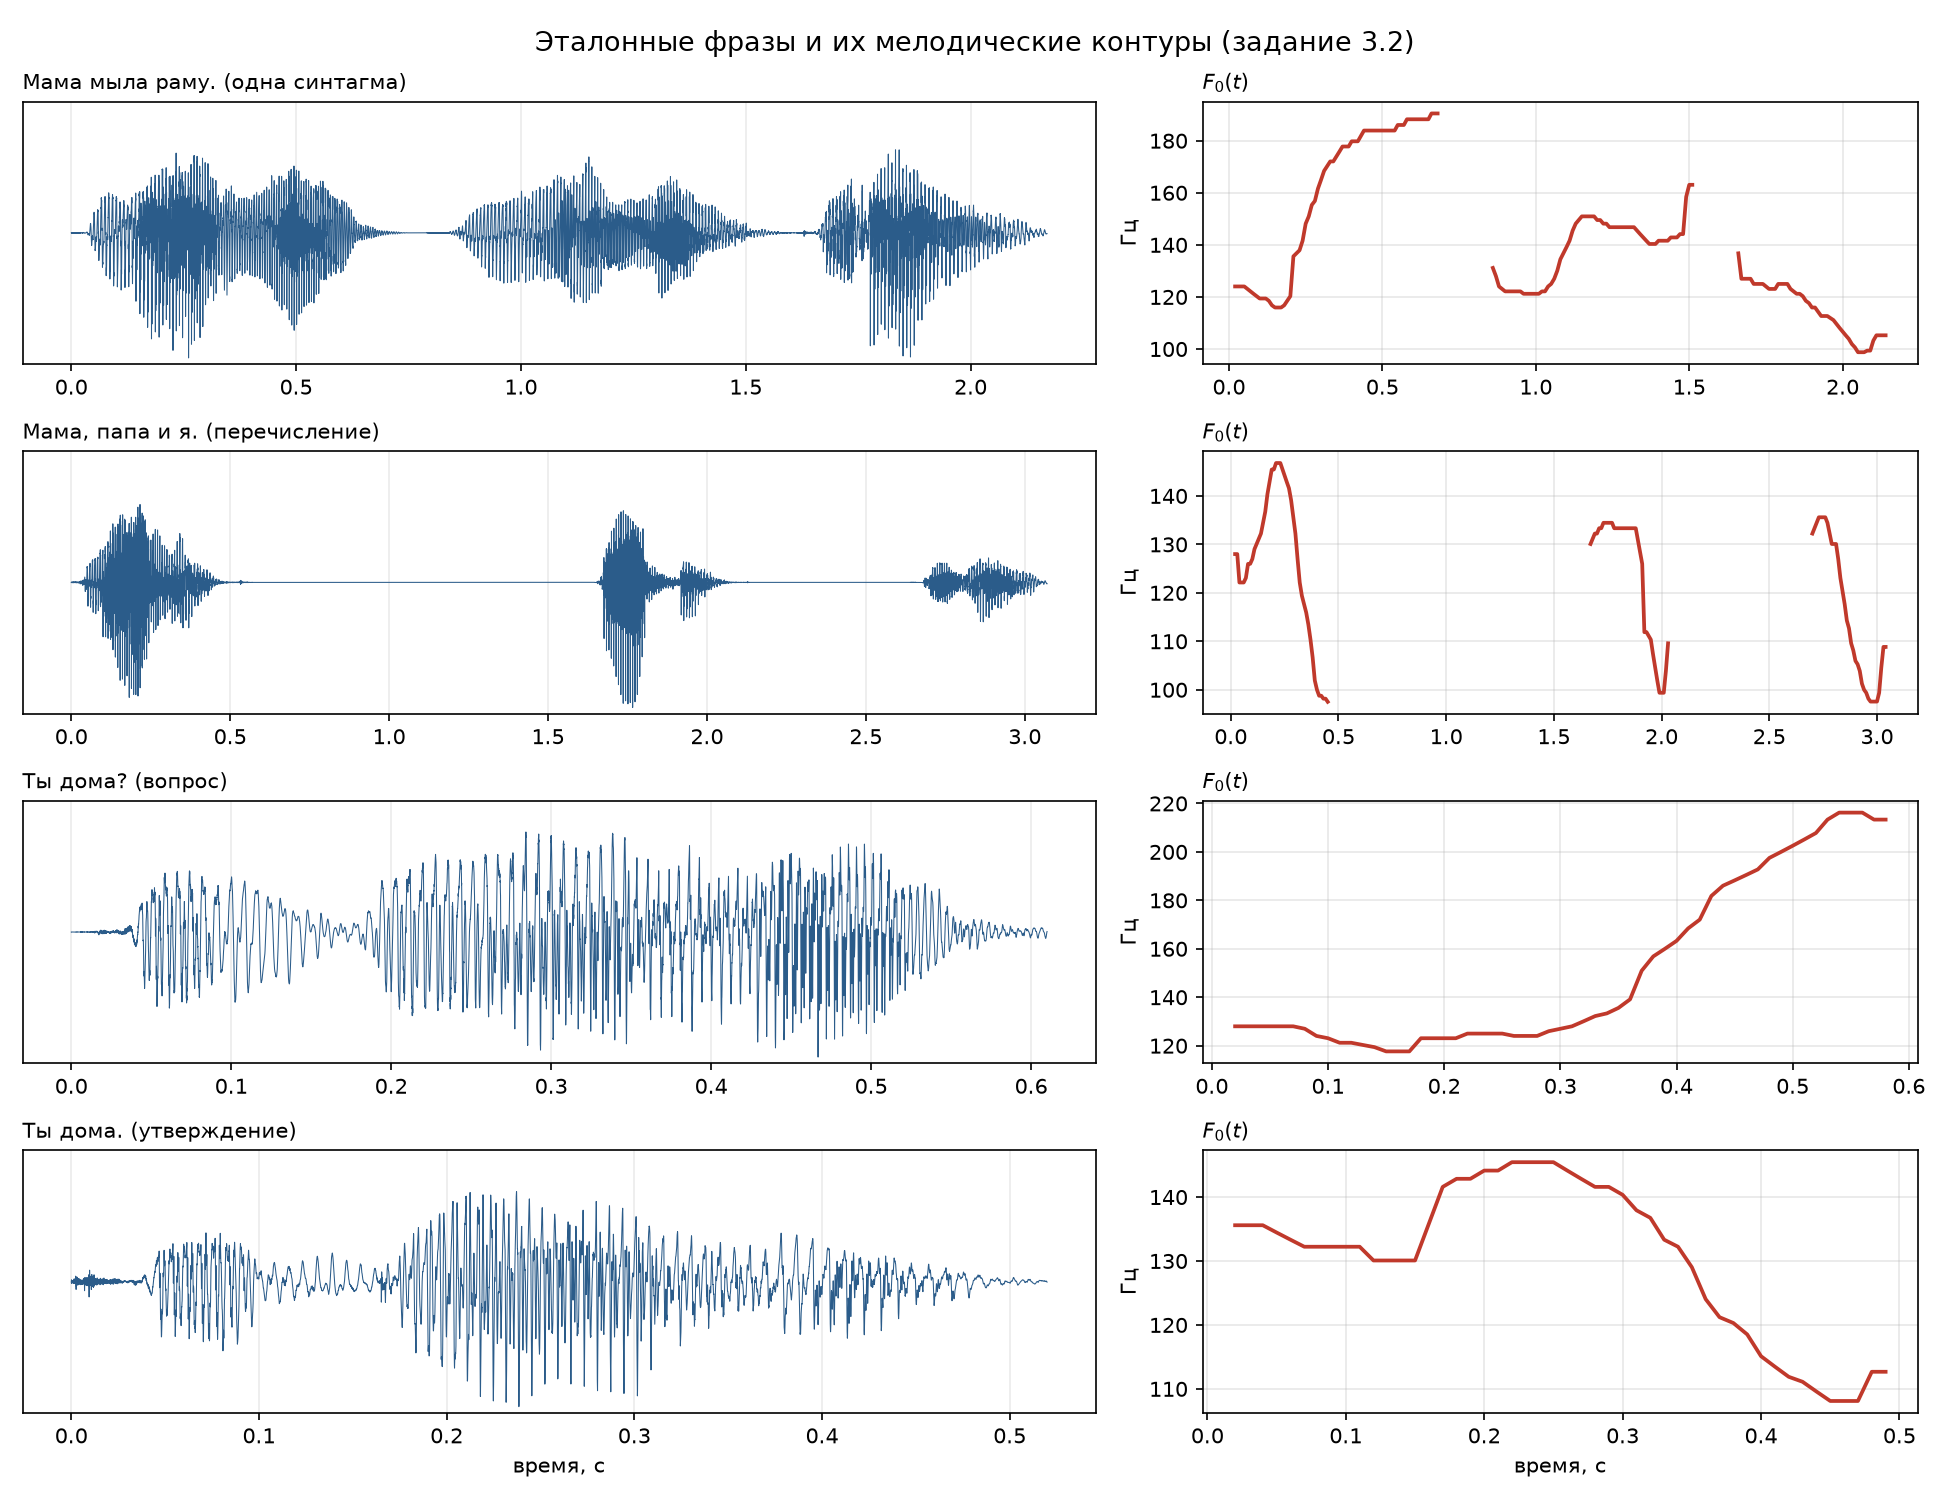
\includegraphics[width=\textwidth]{lab3_reference.png}
	\caption{Осциллограммы эталонных фраз и их мелодические контуры $F_0$}
	\label{fig:reference}
\end{figure}

Фонемная запись фраз (ударный гласный выделен полужирным) имеет вид:
\begin{center}\small
	<<Мама мыла раму.>> $\to$ [\,м \textbf{а} м а~|~м \textbf{ы} л а~|~р \textbf{а} м у\,]\\
	<<Мама, папа и я.>> $\to$ [\,м \textbf{а} м а~|~п \textbf{а} п а~|~и~|~й \textbf{а}\,]\\
	<<Ты дома?>> $\to$ [\,т \textbf{ы}~|~д \textbf{о} м а\,]\\
	<<Ты дома.>> $\to$ [\,т \textbf{ы}~|~д \textbf{о} м а\,]
\end{center}
Буква <<я>> в конце фразы~2 стоит после гласной и по правилам
транскрибирования превращается в пару фонем [й а]. В слове <<дома>>
ударение падает на <<о>>, поэтому фонема [о] является ударной.

Сравнение мелодических контуров эталонных фраз (рис.~\ref{fig:reference})
показывает их принципиальное различие: в вопросе тон повышается к концу
фразы (начало 126~Гц, конец 206~Гц, рост на $+8{,}6$~полутона), тогда как
в утверждении --- понижается (132 \(\to\) 112~Гц, спад на
$-2{,}8$~полутона). Две длинные фразы имеют нисходящий терминальный контур
(спад около $-3{,}7$~полутона). Эти контуры в дальнейшем служат образцом
при просодической обработке синтезированных фраз.
